\documentclass[12pt]{article}
\usepackage{amssymb,amsmath}
\usepackage[pdftex]{graphicx}
\usepackage{epsfig,subfigure}
\usepackage{epstopdf}
\usepackage{bm,url}
\DeclareGraphicsExtensions{.jpg,.pdf,.png,.eps,.ps}
\usepackage[usenames, dvipsnames]{color}
\usepackage{appendix}
\usepackage{ulem}
\usepackage{ifthen}

\newboolean{markup}

\textheight = 522pt
\textwidth = 450pt

\oddsidemargin 0.0in


\newcommand{\Comment}[1]{\textcolor{Blue}{(Comment: #1)}}

\newcommand{\exec}{{Executive Team}}
\newcommand{\shorte}{{ET}}  %abbrev for \exec

%% Define a new 'leo' style for the package that will use a smaller font.
\makeatletter
\def\url@leostyle{%
  \@ifundefined{selectfont}{\def\UrlFont{\sf}}{\def\UrlFont{\small\ttfamily}}}
\makeatother
%% Now actually use the newly defined style.
\urlstyle{leo}

\newcommand\versionnumber{1.10}
\newcommand\collabname{CMB-S4}

\begin{document}
\setboolean{markup}{false}
%\setboolean{markup}{true}
\ifthenelse{\boolean{markup}}{\newcommand\markcolor{red}} {\newcommand\markcolor{black}}


\title{\collabname\ Science Collaboration Bylaws \\ 
\large{Version \versionnumber}}
\date{}
\maketitle

\vfill

\ifthenelse{\boolean{markup}}{ 
  \textcolor{\markcolor}{\begin{center}{\Large PROPOSED AMENDMENTS 007, 008 & 009\\ MARKED-UP VERSION FOR REFERENCE}\end{center}} \vfill}{}

\newpage

\begin{table}[ht!]
%\caption{Version Control Table.  The version number is given as $X$.$Y$, where major amendments are indicated with  increments to $X$, while minor ones increment $Y$. }
\begin{center}
\begin{tabular}{| l | p{3.7in} | c | c |}
\hline
&  & {\bf Date} & {\bf Date}  \\
{\bf Version}  &  \hspace{1.0in} {\bf Purpose/Changes} & {\bf Proposed} & {\bf Ratified} \\
\hline\hline
1.0 & First complete draft after discussions at March 2018 Collaboration Workshop & 03/12/2018 & 03/19/2018 \\ \hline
1.1 & Amendment to Section 3.4 on Governing Board meetings & 09/05/2018 & 11/08/2018 \\ \hline
1.2 & Amendment to Section 9.1 to extend deadline for creation of publication policy & 02/12/2019 & 03/13/2019\\  \hline 
1.3 & Amendments to Sections 8.1, 8.4, and 8.6 of the CMB-S4 Bylaws, regarding postdoc membership & 03/04/2019 & 05/16/2019 \\ \hline
1.4 & Amendments to Section 6, 6.3 on GB elections, deletion of Appendix A (First election procedures) & 03/06/2020 & 04/20/2020 \\ \hline
1.5 & Amendments to Section 9 regarding the speakers and publication policies & 03/06/2020 & 02/05/2021 \\ \hline
1.6 & Amendments to S8.4 for the transition from Postdoctoral to Senior membership, revises``Intended Senior Membership Status" & 01/21/2021 & \\ \hline
1.7 & Amendments to Figure 1 and Section 5.2 & & 04/22/22 \\ \hline
1.8 & Amendments to Sections 1.2, 5.1, 7, and 7.2 and Figure 1 to redefine Technical Working Groups, preserving the intent of unamended Sections 7.2, 9.2, and 9.3 &  & 04/22/22\\ \hline
1.9 & \textcolor{blue}{Amendments to Section 8 to clarify membership types, status qualifiers, and processes} & & \\ \hline
1.10 & Amendments to Sections 2,3.1,3.3,3.4,6.3,7.3-7.7,10.2 to address minor inconsistencies and extend GB attendance requirements to account for extenuating circumstances & 09/15/2021 & 04/22/22 \\ \hline
& & &\\ \hline
\end{tabular}
\end{center}
\label{tab:version}
\end{table}

\thispagestyle{empty}

\newpage

\tableofcontents

%\Comment{ADD COMMENTS WITH $\backslash$Comment\{ \} }

\newpage

\section{Preamble}

The purpose of the \collabname\ Science Collaboration (hereafter the Collaboration) is to conduct a science program centered on the future Stage-4 ground-based cosmic microwave background (CMB) experiment, \collabname. The Collaboration activities include advocating for, and advancing the design of, \collabname. The Collaboration is expected to play a major role in the establishment of the \collabname\ Construction Project (hereafter the Project) and in its operations, and the Collaboration is expected to lead the scientific analysis. \collabname\ will deliver a highly constraining data set with which any model for the origin of the primordial fluctuations---be it inflation or an alternative theory---and their evolution to the structure seen in the Universe today must be consistent. 

This document outlines the Collaboration governance and organization of scientific activities.

\subsection{Collaboration Governance Objectives}

 The structure of the Collaboration was designed to adhere to the following principles:

\begin{itemize}
\item The Collaboration organization will be based on models used in other successful  large DOE- and NSF-supported experiments. 

\item The Collaboration will strive to maximize the scientific return of the experiment, producing high-quality science in a timely manner and promoting full utilization of the data through public data releases after a suitable proprietary period.

\item The organizational structure of the Collaboration will enable broad representation of its members, and encourage consensus in decision making. 

\item All members of the Collaboration will be expected to contribute to the success of the Collaboration and the Project through work on one or more areas of necessary infrastructure. The organizational structure should incentivize Collaboration members to contribute to the advancement of \collabname\  including work on hardware, software, testing, commissioning, operations, common science infrastructure, documentation,  publications,  management tasks and serving in leadership roles.

\item Towards this end, the Collaboration should provide appropriate credit to data analysts and builders of hardware and/or software; provide leadership opportunities and other opportunities to promote career advancement; motivate people to work together towards common goals; and provide a healthy collaboration culture that establishes standards for behavior consistent with high ethical standards.

\item All members will be expected to abide by the \collabname\ Code of Conduct. 

\end{itemize}

\subsection{Definitions}

The \collabname\ Construction Project (the Project) is distinct from the \collabname\ Science Collaboration (the Collaboration). The Project will be responsible for final design and construction of \collabname, which by necessity will have strong oversight from and  report directly to the associated funding agencies and other sources of funding. The Collaboration and Project must work closely together; many Collaboration members are expected to have important roles within the Project, including participating in the Project working groups associated with the various Level 2 subsystems (the Technical Working Groups). The Project ends when construction is completed and operations begin. Operations may be the responsibility of the Collaboration, or may be conducted by a distinct entity working closely with the Collaboration. These Bylaws pertain only to the Science Collaboration and do not specify the structure of, or relationship to, the Project or Operations. 

Throughout this document,  a ``supermajority vote" is defined as a result with more than two-thirds of the votes received in favor of  the motion. ``Supermajority votes'' require approval by two-thirds of the entire voting body. A ``majority vote" requires that more than half the votes received are in favor of the motion.   A ``quorum" for a meeting is defined as the presence of a majority of a body's members.   For collaboration-wide votes, a ``Voting member" is  defined as a Senior member or a Postdoctoral member (see \S\ref{sec:memberrights}). ``{\it Ex officio}" members of a governance body are those whose membership is owing to their roles elsewhere in the Collaboration.  For example, the Science Council Chairs (\S\ref{sec:SC}) are {\it ex officio} members of the Executive Team (\S\ref{sec:exec}).  In these bylaws,  ``Working Groups" are open to all Collaboration members, and ``Councils" have multiple Working Groups reporting to them, while ``Committees" do not.  

\section{Overall Structure}

The governance structure of the \collabname\ Collaboration is illustrated in Figure~\ref{fig:org_chart}.  The Governing Board (GB) provides oversight to an \exec\ (ET) led by two equal co-Spokespersons.  A number of Councils, Committees and Working Groups carry out necessary work to enable the overall science objectives of the Collaboration. The overall scope, selection of, and interplay among these governance entities is described in the remainder of this document. 

\begin{figure}[h!]
\begin{center}
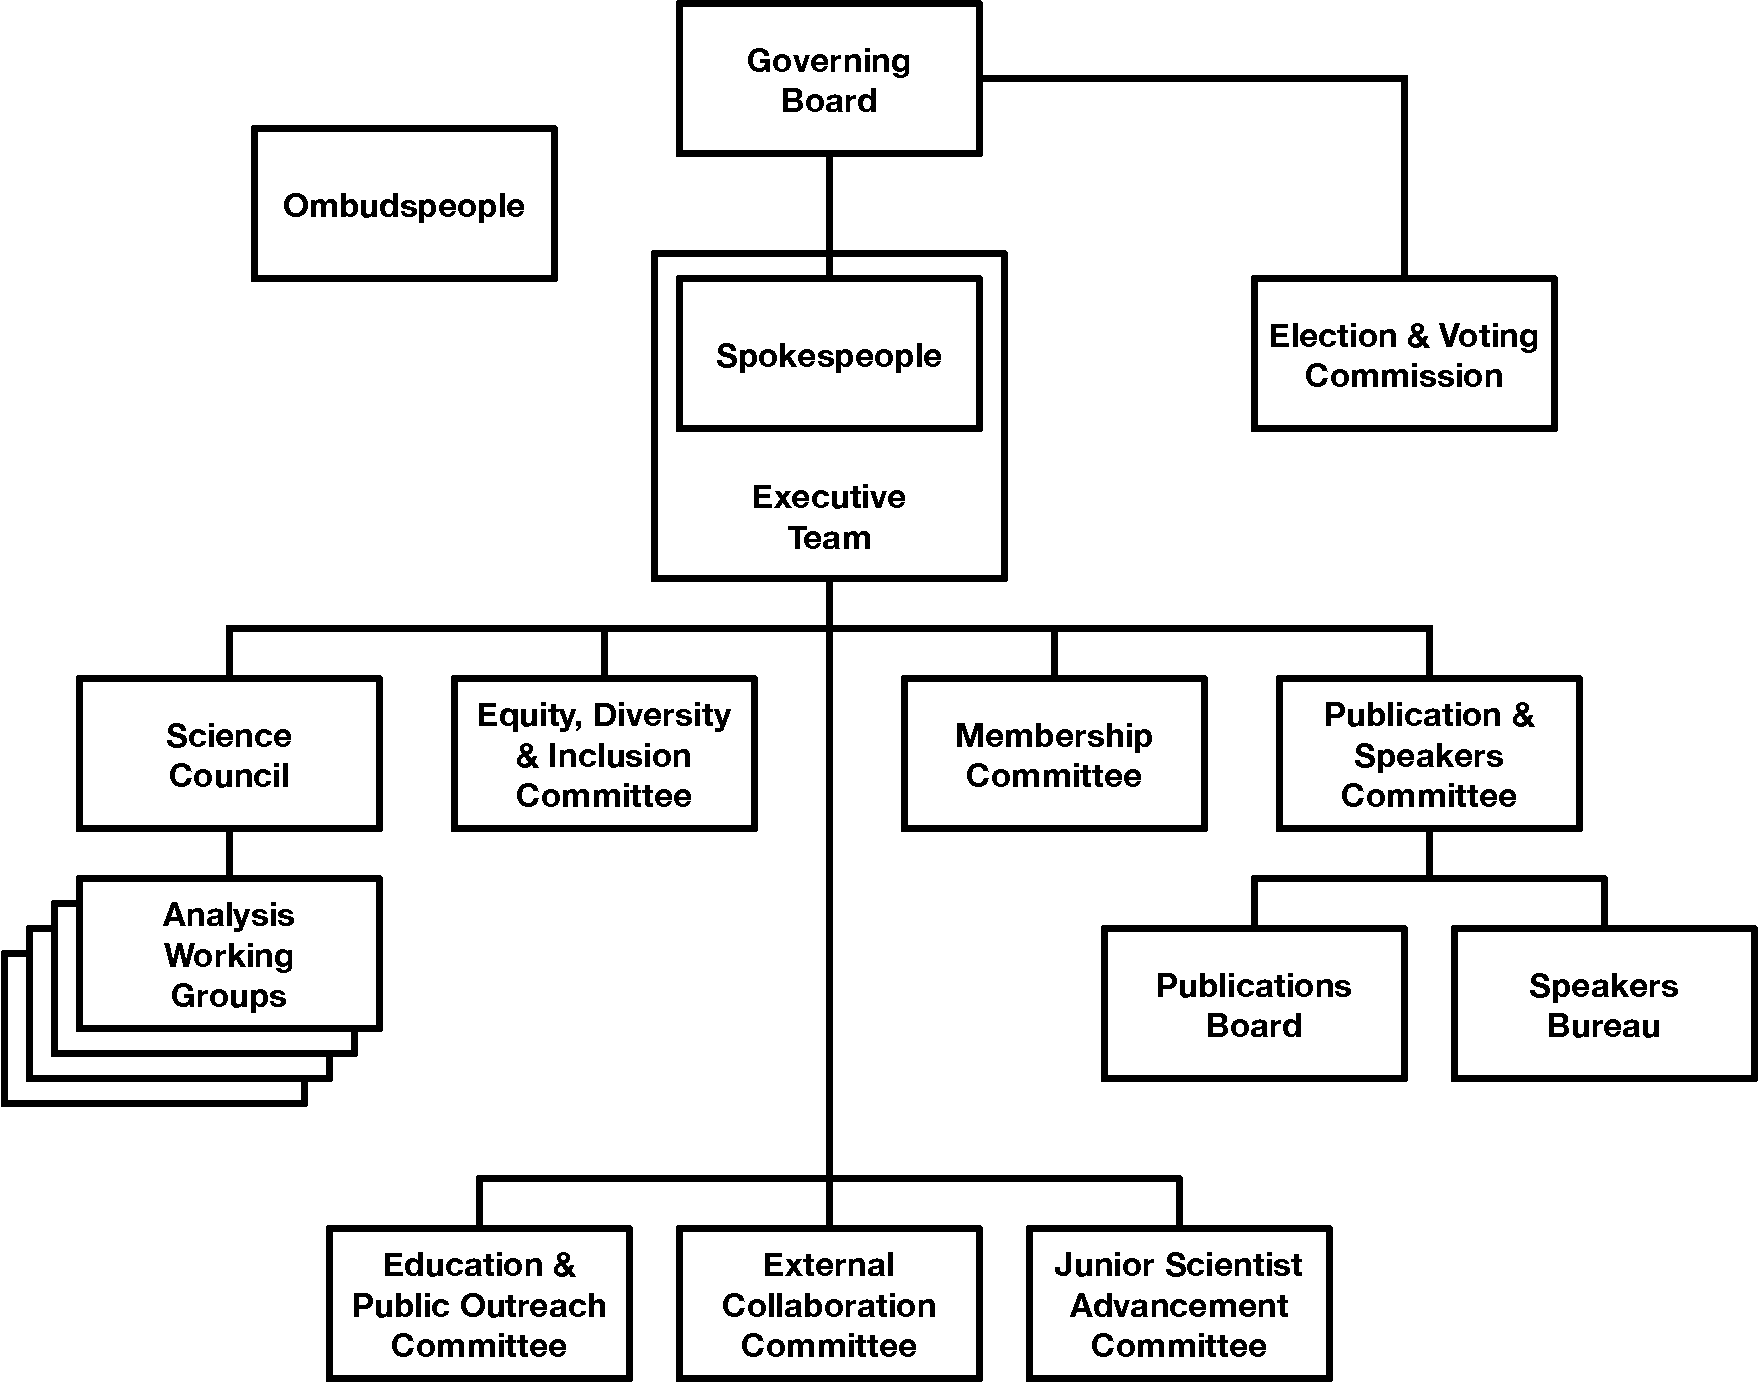
\includegraphics[width=6.5in]{cmbs4_org_v11.pdf}
\end{center}
\caption{\collabname\ Collaboration Organizational Chart. }
\label{fig:org_chart}
\end{figure}

\section{Governing Board}

The Governing Board (GB), a body whose composition is designed to be representative of the membership of the Collaboration as a whole, is the policy-forming body of the Collaboration.  Its other key role is oversight of the Spokespersons.

\subsection{Scope}

Any powers not explicitly assigned to a different governing body in these Bylaws reside in the Governing Board. Governing Board responsibilities include, but are not limited to: 

\begin{itemize}
\item Oversight of the overall progress, status and functioning of the Collaboration.  

\item Oversight of the Spokespersons and their activities.  The GB charges the Spokespersons to prepare a yearly plan for the Collaboration.  The plan must be ratified by a supermajority vote of the GB.  The GB charges the Spokespersons to carry out specific duties for the Collaboration, including, but not limited to, Collaboration reviews, and reviews of the Councils and Committees operating under the auspices of the Spokespersons and the \exec.  The GB may require a detailed verbal, or written report from the Spokespersons on any action. The GB may remove a Spokesperson by a supermajority vote if their performance is insufficient.

\item Approval and revision of Collaboration Bylaws, including the Membership and Publication and Speakers policies. The currently ratified version of the Bylaws must be available on a public website. Amendment of the Bylaws requires a supermajority of the GB.  Major changes (see \S\ref{sec:amend}) must be ratified by the majority of the Voting members of the Collaboration.

\item Formal acceptance of new Collaboration members, and resolution of membership conflicts/issues, such as the removal of members from the Collaboration for failure to perform their duties or serious violations of the Code of Conduct. The change in status of a member (including acceptance or removal) requires approval by a supermajority of the GB.

\item Organization of elections for Spokespersons, GB members, and other elected Collaboration officials (see \S\ref{sec:elections}).  

\item Removal of any Collaboration member from an elected or appointed leadership role in the event of major failings of professional conduct, or gross insufficiency of performance.  Removal requires a supermajority vote of the GB.   Leadership roles include, but are not limited to, the Spokespersons, GB members, \shorte\ members, and Council and Committee members and chairs.

\item Approval of additional long-standing subcommittees. This may include promotion of short-term subcommittees established by the Spokespersons to long-term status. 

\end{itemize}

\subsection{Board Representation}

The GB is composed of 19 members, 18 drawn from the Senior members of the Collaboration and one drawn from the Postdoctoral members (see \S\ref{sec:memtypes}). The Spokespersons and other members of the \exec\ may not serve contemporaneously on the GB. The length of a term of service on the GB is two years for Senior members and one year for the Postdoctoral member; GB members are allowed to serve at most two terms consecutively. To ensure that the board is truly representative of the Collaboration, prior to each GB election,  the GB and the Spokespersons (or the ICCC for the first election) will particularly encourage suitable candidates from a broad range of backgrounds to self-nominate  for GB membership.  Further details on the election of GB members is provided in  \S\ref{sec:gb-elections}.

\subsection{Governing Board Chair, Vice Chair and Secretary}

The GB Chair is responsible for scheduling GB meetings, coordinating requests for reporting from the Spokespersons, distributing the agendas, and chairing the meetings.  The GB Chair only votes on matters before the GB if their vote is needed to break a stalemate.  The GB Vice Chair will preside if the Chair is absent. A GB Secretary will be delegated to take and distribute the minutes to the GB, and provide summaries of the meetings to the Collaboration.   

Every year, starting with the inception of the GB, the Chair and Vice Chair of the GB are elected by the GB from within its membership to serve one-year terms. The Secretary of the GB is chosen informally by the GB Chair to serve during their term. 

\subsection{Governing Board Meetings}

The first Governing Board will establish rules for its meetings after electing its Chair. This first meeting will be held no later than two months after the selection of the GB.  Agendas for scheduled meetings will be available to the full Collaboration in advance.  It is expected that the GB will meet no less than quarterly to ensure adequate attention to its duties. Such meetings will occur approximately twice per year in closed session at every Collaboration meeting and additional meetings will be held by telephone or video conference. The GB Chair may call special meetings as needed. The Spokespersons are typically asked to attend GB meetings, with the exception of any Closed Executive Sessions during the meetings.  The GB Chair can invite other observers at their discretion.

Each meeting requires a quorum to conduct official GB business. Except where a supermajority vote is required, a motion will carry if more than half of the entire GB membership votes in favor of the motion. GB members may cast votes directly or by proxy. GB votes can be held by email or other online method. Summaries of the GB meetings are distributed to the full Collaboration by the GB Chair or GB Secretary. These summaries must include meeting attendance and the results of any votes taken. It is the expectation that GB members participate in the majority of meetings ($\ge 50\%$). However, individual GB members are allowed to request a reduction of the attendance requirement due to extenuating circumstances (e.g., including but not limited to unfriendly time zones, family leave, parental leave, medical leave). The request can be made to the GB Chair and Vice Chair of the GB, who can determine whether to approve the request. If a GB member fails to participate in the agreed number of GB meetings in a year, their seat will be open to election during the following cycle and they will be barred from the board for a two-year term.  


\subsection{Election and Voting Commission}

The GB appoints the Chair and two additional members of the Election and Voting Commission (EVC).  The EVC is charged with conducting elections as spelled out in \S\ref{sec:elections}. The EVC acts independently of the GB, but any points of substantive disagreement amongst the EVC members should be referred back to the GB.  Commission members serve two-year terms ordinarily.  However, the GB may choose to extend the first term of the Chair to  three years, to allow staggering of the membership for improved continuity between commissions.   Commission members may be removed with a supermajority vote of the GB.
 
 \subsection{Removal of members from Leadership Roles}
 
The GB must inform the Collaboration of its decision to remove a member from a leadership role within one working week after the vote to remove.  In the event of a removal of someone from an elected or appointed position, the GB may make an off-cycle appointment or hold a special election to fill the open position quickly, or wait until the next election cycle.  

\section{Co-Spokespersons}
\label{sec:spokes}

\subsection{Scope}

The leadership of the Collaboration resides with two equal co-Spokespersons. Each Spokesperson participates actively in the management of all aspects of the Collaboration and, as the executive officials of the Collaboration, both  are responsible for its day-to-day management. To carry out their duties, the Spokespersons are expected to solicit advice from the \exec, the GB and the Collaboration at large.   

The Spokespersons may appoint up to two members of the \exec. This appointment flexibility will enable the Spokespersons to obtain expert advice on an as-needed, short-term basis for matters including (but not limited to) technical and managerial topics.
Such appointees require approval by the GB, and may be removed from the \exec\ at the Spokespersons' discretion.  Appointments are limited to two years, but may be renewed with approval of the GB. 

Spokesperson responsibilities include, but are not limited to, the following: 
\begin{itemize}
\item Submitting a yearly plan for the Collaboration to the GB for approval. 
\item Serving as the primary interface of the Collaboration with the Project, partnering institutions, the government agencies, private and public funding institutions, scientific organizations, and the media. Reports on such activities will be provided on a semi-annual basis or by request to the GB.
\item Ensuring public dissemination of scientific results. 
\item Creation of short-term ad hoc committees for the purpose of such tasks as creation of review materials, white papers, exploration of new partnerships, etc.
\item Organizing and running Collaboration meetings. 
\item Ensuring that the Collaboration public and private websites are maintained, including the posting of all governance roles and responsibilities, and Collaboration documents. 
\item Carrying out other duties as charged to them by the GB. 
\end{itemize}

Spokespersons are elected to two-year terms and are limited to two consecutive terms. The election process is detailed in \S\ref{sec:elections}. 

\section{\exec}
\label{sec:exec}

\subsection{Scope}

The \exec \ (\shorte) is an elected and appointed board led by the Spokespersons. It consists of up to 10 members: the Spokespersons, the co-Chairs of the Science Council,  the Chair of the Membership Committee, the Chair of the Publication and Speakers Committee, the two co-Chairs of the Equity, Diversity and Inclusion Committee, and up to two members appointed by the Spokespersons. The ET is the agile decision-making body in the Collaboration with the ability to address the day-to-day collaboration issues.  The \shorte\ is structured to facilitate the flow of information to the Spokespersons from the Collaboration and vice versa, as well as to provide a sounding board for the Spokespersons.

The \exec \ has three main roles:
\begin{itemize}
\item to provide leadership on scientific, membership, financial, and organizational decisions and issues. The decisions will ultimately be made by the Spokespersons, but will be discussed and reasoned through the \exec.  In the event that the Spokespersons do not agree on a particular topic, the \shorte\ will hold a vote requiring only a majority.
\item to ensure Spokesperson decisions are made in the best interests of the Collaboration.  Any two \shorte\ members may call for a vote on any topic, and if $\geq 50\%$ of the \shorte\ is in disagreement with proposed activities of the Spokespersons, the issue is referred to the GB for further discussion. 
\item to aid the Spokespersons in being the Collaboration liaisons to the Project.
\end{itemize}

\subsection{\exec \ Meetings}

The Spokespersons will chair the meetings, provide the agendas, and establish rules for the \shorte\ meetings. The first meeting will be held no later than two weeks after the election of the Spokespersons and the Council and Committee Chairs. It is expected that the \shorte\ will meet no less than twice a month to ensure adequate attention to its duties. Meetings can be called on the initiative of a Spokesperson or at the request of an \shorte\ member, provided that a Spokesperson agrees. ET meeting agendas will be made available to the Collaboration.

Each meeting requires a quorum to conduct official \shorte\ business.  It is the expectation that \shorte\ members participate in the majority of meetings; \shorte\ members who fail to participate in a majority of meetings over a one-year period will be replaced in the nearest election cycle and barred from the \shorte\ for a two-year term.  

\section{Elections}\label{sec:elections}

All elected positions in the CMB S4 Collaboration serve two-year terms (with the exception of the Postdoctoral member on the GB, who serves a one-year term). Most positions have term limits.  Elections for GB members are  arranged so that $\sim 50\%$ of the members will be up for election each year. New appointments take office on July 1 in the year of their election.  

As there are restrictions on the overlap of elected officials between various governing bodies, elections are timed to provide Collaboration members multiple opportunities to participate in Collaboration governance. In a given election year the ordering proceeds as follows: elections are held first for the Spokespersons, as needed. Next, elections are held for the Science Council co-Chairs, Membership Committee Chair and the Publication and Speakers Committee Chair, as needed.  A third election is held to fill available positions for the Governing Board. Elections for positions outside the top levels occur when required as such officials are not prohibited from serving other elected roles. 

Each candidate provides a Candidate Statement to the EVC, which makes them available to the Collaboration via the \collabname\  internal web page prior to the balloting. Votes are cast anonymously online by Voting members, with the elections managed by the EVC, and timed to permit adequate time to evaluate the slates of nominees for each election and still assure the new appointments are able to take office on July 1.  The EVC, in consultation with the GB,  determines the detailed timing of the balloting and determines procedures for dealing with any election situations not anticipated in the Bylaws.

\subsection{Spokespersons}

Spokespersons are elected to two-year terms. All Senior members (see \S\ref{sec:memtypes}) may run for these positions.  If a member of the GB is elected as a Spokesperson, they must resign their GB seat prior to the start of their Spokesperson term and this vacancy will be filled in the next GB election. 

Prior to the election, Voting members are asked to nominate individuals for Spokesperson to the Election and Voting Commission. Each Voting member may nominate candidates and self-nominations are accepted. After a nomination period, the EVC consults with the nominees to ascertain their willingness to stand for the election.

A ranked voting scheme approved by the GB prior to the election is used to determine the Spokespersons.  Adoption of a ranked voting scheme that differs from that used during the previous election requires approval of a supermajority of the GB.  Elections are to be held sufficiently early such that new electees may interact with the current Spokespersons and \shorte\ for three months prior to taking office to ensure a smooth transition. In the event of a tie preventing selection of two Spokespersons, a runoff election will be held to choose among the candidates with the same ranking. 

\subsection{Council and Committee Chairs}

The co-Chairs of the Science Council, and the Chairs of the Membership Committee and the Publication and Speakers Committee are elected to two-year terms. All Senior members (see \S\ref{sec:memtypes}) may  run for these positions.  If a Voting member of the GB is elected to one of these positions, they must resign their GB seat prior to taking office as Chair, and this vacancy will be filled in the next GB election. 

Prior to the election, Voting members are asked to nominate individuals for the Chair positions to the EVC. Self-nominations are accepted. After a nomination period, the EVC consults with the nominees to ascertain their willingness to stand for the election. Candidates are only allowed to stand for one open position in a given election.  

A ranked voting scheme approved by the GB prior to the election is used to determine the Science Council Co-chairs. Adoption of a ranked voting scheme that differs from that used during the previous election requires approval of a supermajority of the GB. In the event of a tie, a runoff election will be held to choose among the candidates with the same ranking.

\bigskip
\subsection{Governing Board}
\label{sec:gb-elections}

The 18 GB members drawn from the Senior members of the Collaboration are elected to two-year terms. Elections for GB members are arranged so that 50\% of the members will be up for election each year. All Senior members may run for these positions. The one GB member drawn from the Postdoctoral members of the Collaboration is elected for a one-year term. Prior to each election, the current GB will define various representation requirements that it deems important to include on the GB (possibly including, e.g., tenure-track and early career scientists,  historically underrepresented groups, members from partner countries with significant membership, members of small institutions, representatives of existing CMB programs, etc.); no more than 50\% of the open seats on the board in an election can be reserved for such requirements.

The election for the Senior members on the GB proceeds as follows. 
Prior to the election, Voting members are asked to nominate individuals for the GB to the EVC. Self-nominations are accepted. After a nomination period, the EVC consults with the nominees to ascertain their willingness to stand for the election. A ranked voting scheme approved by the GB prior to the election is used for the GB election. Adoption of a ranked voting scheme that differs from that used during the previous election requires approval of a supermajority of the GB. The EVC will synthesize the voting results to provide a ranked list of all the candidates to the GB. 

Half of the open seats (or the closest number greater than 50\% of the total in the case of an odd number of vacancies) are automatically filled by the top-ranked candidates. If the representation requirements outlined above are unfulfilled by the elected candidates, the remaining open seats will be filled by the ranked-order voting results list until the number of remaining unfilled seats equals the number needed to meet the representation requirement.  At this point, the first rank-ordered candidate who meets one of the remaining unfulfilled requirements is selected. The process will be repeated until all seats are filled. In the case where a candidate withdraws after the election process has begun, the candidate will be ignored in counting ballots, and votes will move to the next choice on the ballot. Continuing GB members (those whose seats are not open) will adjudicate any election issues, in consultation with the EVC.

The election for the Postdoctoral member of the GB follows the same procedure, with the exception that only Postdoctoral members are eligible to both nominate and vote for candidates for this position.

If a GB member, including a Postdoctoral member, resigns or is removed outside of the elections period and more than six months before the end of the member's term, a special election will be held to fill the seat for the remainder of the member's term.

\subsection{All Other Elected Positions}

For other elected Collaboration roles, the EVC is charged with establishing election rules and conducting these elections. Note that the EVC cannot make voting requirements more restrictive than those for the ET (including Spokespersons and Council and Committee chairs) and GB elections. Terms of elected positions are limited to durations of at most two years. 

\section{Councils and Committees}
\label{sec:councils}

Three of the organizational structures overseen by the Spokespersons have representatives on the \exec\ as described in \S\ref{sec:exec}.  These are the Science Council, the Membership Committee, and the Publications and Speakers Committee.  Their composition and charges are described in this section.  Three other standing committees for the Collaboration are also described below.  

\subsection{Science Council and Analysis Working Groups}
\label{sec:SC}

The Science Council works closely with the Spokespersons to coordinate the key scientific objectives of the Collaboration.  The Science Council is led by two co-Chairs elected by the Voting members of the Collaboration, who also serve as members of the \exec. The Science Council chairs serve two-year terms and are limited to two consecutive terms with one year off required before standing again.
The remaining members of the Science Council are the co-coordinators of the various Analysis Working Groups. These Working Groups are open to all Collaboration members, and will be formally established by the Spokespersons.  

The Science Council approves the projects that lead to publications and is responsible for maintaining a list of Key Science topics  (\S\ref{sec:pubprop}). It is charged to work closely with the Spokespersons and the \shorte\ to produce a coherent plan for advancing the key science goals of the Collaboration and to work towards the successful execution of this plan.

Each Analysis Working Group will have two co-coordinators who  serve for two-year terms with the exception of one initial coordinator who will serve for a three-year term to enable staggered appointments in the future.  The Science Council Chairs will solicit self-nominations for these co-coordinator positions. The Spokespersons will appoint coordinators with the advice of the Science Council Chairs, and will consider the distribution of early- and late-career members when making these appointments. Coordinators will ordinarily not serve back-to-back terms.\\


\subsection{Membership Committee}

The Membership Committee (MC) consists of seven people including a Chair. The Chair is elected following the election cycle of the Collaboration with a  two-year term, and is limited to two consecutive terms with one year off required before standing again. The six remaining members are appointed by the Spokespersons after consultation with the \shorte\ and subject to approval of the GB. Appointments of MC members are staggered so that 50\% are appointed each year. These members have the same term duration and limits as the elected Chair. If a MC member leaves before their term is complete, the Spokespersons will appoint a replacement to complete their term, subject to approval of the GB.   MC members can be removed by a supermajority of the GB at any time.  

The appointed members of the MC should represent the overall Collaboration, and there should be at least two members from the Technical Working Groups and two members from the Analysis Working Groups on the MC.  This balance may be amended as the scientific needs of the Collaboration evolve. 

The duties of the MC  are to review and evaluate membership applications, review annual activity reports, and recommend changes in membership status. The MC maintains an up-to-date list of all Collaboration members, available on a public website.  The MC in consultation with the \shorte\ works with applicants and continuing members to identify roles and infrastructure tasks that add value, avoid redundancy, and make the Collaboration as efficient as possible.

\subsection{Publication and Speakers  Committee}
\label{sec:pubcouncil}

The Publication and Speakers Committee (PSC) consists of thirteen people including the Chair. The Chair is elected following the election cycle of the Collaboration with a two-year term, and is limited to two consecutive terms with one year off required before standing again. There are two subcommittees which together comprise the PSC: the Publications Board with eight Collaboration members and the Speakers Bureau with four Collaboration members. The Chair of the PSC chairs both subcommittees. The twelve non-elected committee members are appointed by the Spokespersons after consultation with the \shorte\ and subject to approval of the GB. Appointment of PSC members are staggered so that 50\% are appointed each year. The twelve appointed members serve with the same term duration and limits as the Chair. Roughly half of each group should be pre-tenure or the equivalent junior status for non-professorial positions. If a PSC member leaves before their term is complete, the Spokespersons
will appoint a replacement to complete their term, subject to approval of the GB. PSC members can be removed by a supermajority of the GB at any time.  

\subsection{Junior Scientist Advancement Committee}

The role of the Junior Scientist Advancement Committee (JSAC) is to ensure that junior members (defined as Student members and Postdoctoral members; see \S\ref{sec:memtypes}) within the Collaboration are represented, assisted, and supported throughout the  tenure of the Collaboration. This will include arranging mentors for junior members who desire mentorship, and facilitating junior member career advancement through relevant workshops and other activities. The JSAC Chair and Vice Chair are appointed by the Spokespersons after consultation with the \shorte\ and subject to approval of the GB. It is expected that either the Chair or Vice Chair (or both) be Senior members of the Collaboration.

The Chair and Vice Chair serve two-year terms that parallel the Collaboration election cycle, and are limited to two consecutive terms with one year off required before standing again. Membership on the JSAC is open to volunteers from the Collaboration, with the approval of the JSAC Chair, after solicitation of nominations from the full Collaboration. JSAC members serve for two-year terms. Consecutive terms are allowed.


\subsection{External Collaborators Committee}

The role of the External Collaborators Committee (ECC) is to provide the necessary link to external follow-up observations or survey data that are required to maximize the science return from \collabname. The ECC Chair and Vice Chair are appointed by the Spokespersons after consultation with the \shorte\ and subject to approval of the GB.  

The Chair and Vice Chair serve two-year terms that parallel the Collaboration election cycle, and are limited to two consecutive terms with one year off required before standing again. The Chair will appoint additional members as required to ensure adequate knowledge of the collaborations being pursued resides in the ECC. Self nominations for consideration for membership on the ECC are expected after solicitation of nominations from the full Collaboration.  

The committee drafts the necessary documents for external collaboration agreements and memoranda of understanding (MOUs). These are presented to the Spokespersons and the \shorte\ who have the authority to amend and alter the agreements and MOUs. The agreements are brought forward by the Spokespersons to the GB for final approval.

\subsection{Education and Outreach Committee}

The Education and Public Outreach (EPO) Committee is responsible for initiating, overseeing, and recording the Collaboration's efforts in the areas of public outreach and education. Its mission is to disseminate Collaboration results to the public and increase general scientific literacy. The committee is overseen by the \exec \ and members are appointed by the Spokespersons after solicitation of nominations from the full Collaboration and after consultation with the \shorte.

The Chair is appointed by the Spokespersons after consultation with the \shorte\  and is limited to two consecutive terms with one year off required before standing again.Terms on the EPO Committee are for two years. Consecutive terms are allowed.  A presentation of EPO efforts and written documentation of activities must be provided to the \shorte\ at each Collaboration meeting or when requested by the \shorte.   

\subsection{Equity, Diversity, and Inclusion Committee}
The Equity, Diversity, and Inclusion (EDI) Committee is responsible for initiating, guiding, and documenting the collaboration's efforts and coordinating with the project to create and uphold a safe, welcoming, and open community. Activities include but are not limited to advocating for policies that promote justice, equity, diversity and inclusion; assessing the collaboration climate to inform recommendations and track progress; empowering collaboration members to remove barriers and contribute to an inclusive and welcoming community; and researching and exploring best practices for equitable organizations.

The committee has two Co-chairs that share equal responsibilities and are appointed by the Spokespersons after consultation with the ET and the GB. Chair term appointments are staggered to maintain continuity. Chair terms are for two years (with one initial three-year term to allow staggered appointments) and are limited to two consecutive terms with one year off required before standing again. The chairs of the EDI committee sit on the ET. Membership on the committee is open to anyone in the collaboration at any stage in their career. Collaboration members are welcome to join the EDI committee by joining meetings and the mailing list at any time. Periodic solicitations for self-nominations to the committee will be advertised to further encourage participation.

\section{Membership Policy}

The Collaboration consists of Ph.D. scientists, engineers, Ph.D. thesis students and others who contribute significantly to the \collabname\ program. Membership conveys certain rights as described below, but comes with the obligation of an ongoing commitment of a substantial fraction of members' research time to the \collabname\ program. \\

{\color{blue}

\noindent STRIKE ALL ITALICISED BLUE TEXT \\

{\it
{\large \noindent 8.1 Membership Types}\\

Five types of members are defined here.  
\begin{itemize}

\item {Senior Member:} A Senior Member of the Collaboration is a member who has a permanent appointment or an appointment, that under normal circumstances can be expected to be renewed indefinitely.   This includes tenure-track appointments at universities and their equivalents elsewhere.  

\item {Postdoctoral Member:} A postdoc working with a Senior Member at their institution can be designated as a Postdoctoral Member by that Senior Member. Postdocs that are not working closely with a Senior Member (hereafter referred to as ``Independent Postdocs'') can apply to become a Postdoctoral Member and have their application evaluated by the Membership Committee on a case-by-case basis.

\item {Student Member:} A graduate student working with a Senior Member at their institution can be designated as a Student Member by that Senior Member.  We do not anticipate granting membership to students who are not supervised by a Senior Member.


\item {Provisional Member:}  A Provisional Member has not yet been approved for Senior, Postdoctoral or Student Member status.  This status applies to all new Student and Postdoctoral Members (including, for example, those in an existing Senior Member's group) as well as potential Senior Members.  This is intended to be a temporary status, typically a year, allowing the Provisional Member to demonstrate sufficient constructive engagement with the Collaboration.

\item {Legacy Member:}  A Legacy Member is a former member who contributed in a key manner to the Project or analysis infrastructure, but is no longer engaged with the Collaboration and is therefore no longer a member.  This status is intended to convey authorship rights to such former members, and to bypass the normal membership procedures should they wish to re-engage with the Collaboration.

\end{itemize}

{\large \noindent 8.2 Membership Rights}\\

Herein, ``Members'' refers to Senior, Postdoctoral, Student and Provisional Members (but not Legacy Members) unless otherwise qualified.  

\begin{itemize}

\item Senior and Postdoctoral Members are Voting Members.  Voting Members  have the right to vote to ratify Bylaws and amendments to Bylaws, and vote in elections for Spokespersons, Governing Board representatives, and the elected positions including the Chairs of the Science Council, and the Membership and Publication and Speakers Committees.   

\item Members have full data access, including during the proprietary period for data that are eventually released.

\item Members (including Legacy Members) have the right to be listed as a co-author on \collabname\ publications as specified in the Publication Policy.

\item Members have access to computational resources designated for \collabname, according to the policies of the relevant Computational Resources Working Group.

\end{itemize}

{\large \noindent 8.3 Membership Requirements}\\

Members must commit effort to approved infrastructure tasks. The Membership Committee will work with the \exec\ to define and recommend infrastructure tasks that need filling, and to define and communicate with Members the level of expected effort. Tasks can include,  for example, designing, building, and testing software, hardware, or simulations; contributing to commissioning and observations; and management tasks.  Just as for the hardware, we anticipate having a collaboration-wide architecture for the software.  Thus, Members are expected to comply with interface, documentation and code review requirements in support of the goals of the Collaboration.   Other ways of contributing include taking on roles in the governance, including membership on the GB, EVC, ET, or the Councils and Committees described in \S\ref{sec:councils}.\\

{\large \noindent 8.4 Membership Application and Approval Process}\\

After the Collaboration is formed with a first set of initial members (see \S\ref{sec:initmembership}), the process for membership to \collabname\ will be as specified below.

\begin{itemize}

\item Potential Senior Members will apply for Provisonal Membership via a written application where they specify their proposed work on \collabname. Applicants who have already made significant contributions to CMB-S4, either as a postdoctoral member or as a non-member, may be recommended for non-provisional (regular) Senior membership by the Membership Committee.


\item Potential Independent Postdocs can apply for Postdoctoral Membership and have their applications reviewed on a case-by-case basis.
  
\item Postdoctoral members can request Òintended senior membership statusÓ when applying to permanent positions by submitting a proposed research plan to the Membership Committee. If approved, they can request a letter from the Spokespersons describing their relationship to CMB-S4 to include in their application packages, or to pass to their letter writers.  Intended senior members who successfully transition to a permanent position are expected to follow the normal application process for provisional senior membership.

\item Applications are reviewed by the Membership Committee. The Membership Committee recommends membership to the Governing Board.  The Governing Board approves membership.

\end{itemize}

{\large \noindent 8.5 Initial Membership}\\

The Collaboration will initially consist of members that were eligible to vote on these governance Bylaws (by virtue of attendance at two or more Collaboration meetings, or a successful petition for eligibility), and did cast a vote on them. Within the first year of the Collaboration's establishment, prospective members can be granted membership by successfully petitioning the Membership Committee despite not satisfying the above criteria.  The Membership Committee may approve such applications during the first year without action by the Governing Board.  

{\large \noindent 8.6 Membership Review and Changes in Status}\\

The membership status of each member will be reviewed by the Membership Committee each year. 

\begin{itemize} 

\item Each Senior Member and each Independent Postdoc will submit an annual activity report to the Membership Committee. Reports of the Senior Members should include discussion of the activities of their supervisees (e.g., postdocs and students) in their report. The Membership Committee will review those reports, consulting with Collaboration members and Working Group leaders as appropriate.
  
\item Provisional Members will submit an annual activity report to the Membership Committee, which will review the report and determine whether the Provisional Member should be promoted to a Senior Member status, continue as a Provisional Member, or have their membership revoked.  Provisional Membership is intended to be a temporary status.

\item Members leaving the Collaboration may be granted Legacy Membership upon review by the Membership Committee and approval by the GB.

\item The Governing Board has the authority to grant or terminate all forms of membership.

\item If the effort of any Member appears insufficient, the Membership Committee will consult with the Spokespersons to develop a plan to remedy the situation.  If needed, the Spokespersons will work with the Membership Committee to prepare a recommendation to the GB for corrective action, including suspension or termination of membership.   This can also be done should the Membership Committee deem the actions of a Member to have been egregious and detrimental to the Collaboration.

\item When a person's membership in the Collaboration ends, they will no longer have access to the \collabname\ document and database repository, internal forums, computing resources and data.  Authorship rights will continue, or not, as prescribed in the Publication Policy bylaws.

\end{itemize}

}


\newpage

\noindent REPLACE ABOVE WITH FOLLOWING BLUE TEXT

\subsection{Membership Types}
\label{sec:memtypes}

Four membership types and four status qualifiers are defined here. \\

\noindent The four membership types are:
\begin{itemize}

\item {\bf Senior Member:} 
A Senior member of the Collaboration is a member who has a permanent appointment or an appointment that, under normal circumstances, can be expected to be renewed indefinitely.  This includes tenure-track appointments at universities and their equivalents elsewhere.  

\item {\bf Postdoctoral Member:} 
A Postdoctoral researcher working with a Senior member at their institution can be designated as a Postdoctoral member by that Senior member. Postdoctoral researchers that are not working closely with a Senior member can apply to become an Independent Postdoctoral member. Postdoctoral membership is limited to the term of the appointment, after which the individual's membership must be renewed according to their new status.

\item {\bf Student Member:} 
A graduate student working with a Senior member at their institution can be designated as a Student member by that Senior member.  We do not anticipate granting membership to students who are not supervised by a Senior member. Student membership is limited to the expected term of the studentship, after which the indiviual's membership must be renewed according to their new status.

\item {\bf Legacy Member:}  
A Legacy member is a former Senior or Postdoctoral member who has made especially notable contributions to the Project and/or Collaboration, but is no longer engaged with the Collaboration. This exceptional status is granted by the Governing Board and is intended to convey authorship rights to such former members, and to bypass the normal membership procedures should they wish to re-engage with the Collaboration.

\end{itemize}

\noindent
The four status qualifiers are:

\begin{itemize}

\item {\bf Full:}
This is the normal membership type, assumed unless otherwise specified in these bylaws.

\item {\bf Provisional:} 
New Senior, Postdoctoral and Student members will normally start with a Provisional status. This is intended to be a temporary status allowing the Provisional member to demonstrate sufficient constructive engagement with the Collaboration. New members who have already made substantive contributions to CMB-S4 may be deemed to have demonstrated sufficient engagement and be appointed as Full members. \sout{Provisional Postdoctoral and Student members who were designated as members by a Provisional Senior member may not be raised to Full status before that Senior member.}

\item {\bf Pending:} 
Postdoctoral and Student members whose membership term has expired, but whose membership has not yet been renewed, will be moved into Pending status. If the renewal would involve a change of membership type (from Student to Postdoctoral or Senior, or from Postdoctoral to Senior) then this status will afford them the intersection of the rights of the old and new membership types.

\item {\bf Inactive:}
Members who are deemed to be insufficiently engaged with the Collaboration, or who have failed to respond to requests for Annual Activity Reports or Membership Renewals in a timely manner, may be moved to Inactive status by the Membership Committee. A return to the member's prior status will be considered when the appropriate Annual Activity Report or Membership Renewal is submitted in writing to the Membership Committee. Inactive members retain their membership rights, but will typically be removed from the membership list, at the discretion of the Governing Board, after one year.

\end{itemize}

\subsection{Membership Rights}\label{sec:memberrights}

Herein, ``members'' refers to Senior, Postdoctoral and Student members (but not Legacy members) unless otherwise qualified.  

\begin{itemize}

\item Senior and Postdoctoral members are Voting members.  Voting members  have the right to vote to ratify Bylaws and amendments to Bylaws, and vote in elections for Spokespersons, Governing Board representatives, and the elected positions including the Chairs of the Science Council, and the Membership and Publication and Speakers Committees. 

\item Members have full data access, including during the proprietary period for data that are eventually released.

\item Members (including Legacy members) have the right to be listed as a co-author on \collabname\ publications as specified in the Publication Policy.

\item Members have access to computational resources designated for \collabname, according to any policies of the Collaboration and/or Project.

\end{itemize}

\subsection{Membership Requirements}

Members must commit effort to approved infrastructure tasks. The Membership Committee will work with the \exec\ to define and recommend infrastructure tasks that need filling, and to define and communicate with members the level of expected effort. Tasks can include, for example, designing, building, and testing hardware and software; generating or analyzing simulations; developing science requirements and associated theoretical studies; contributing to commissioning and observations; and management tasks. Just as for the Project hardware and software, we anticipate having Collaboration requirements on the analysis software; members are expected to comply with interface, documentation and code review requirements in support of the goals of the Collaboration. Other ways of contributing include taking on roles in the governance, including membership on the GB, EVC, ET, or the Councils and Committees described in \S\ref{sec:councils}.

\subsection{Membership Application and Approval Process}

The process for being taken into membership of \collabname\ is as follows:

\begin{itemize}

\item Potential Senior and Independent Postdoctoral members apply for membership via a standard written application in which they specify their past and proposed work on \collabname. All applications are reviewed by the Membership Committee, which makes recommendations to the Governing Board for its approval. Typically, approved members will be given Provisional status, but applicants who have already made significant contributions to CMB-S4, either as a Postdoctoral or a Student member, or as a non-member, may be recommended for Full status by the Membership Committee.

\item Supervised Postdoctoral and Student members may automatically be designated for membership by their supervisor, with such designation including the term of the postdoctoral appointment or expected term of the studentship.

\end{itemize}

Postdoctoral members who are applying for positions that would qualify them for senior membership may apply for Intended Senior member status by submitting a proposed research plan to the Membership Committee. If approved, they can request a letter from the Spokespersons describing their relationship to CMB-S4 to include in their application packages, or to pass to their letter writers.  Intended Senior members who successfully transition to a permanent position are expected to follow the normal application process for provisional senior membership.

\subsection{Membership Review and Changes in Status}

The membership status of each member will be reviewed by the Membership Committee each year; the Governing Board retains the authority to grant or terminate all forms of membership.

\begin{itemize} 

\item Each Senior member and each Independent postdoc will submit an Annual Activity Report to the Membership Committee. Senior members should include discussion of the activities of their Postdoctoral and Student member supervisees in their report. The Membership Committee will review these reports, consulting with Collaboration members and Working Group leaders as appropriate.
  
\item The Annual Activity Reports will be used by the Membership Committee to determine: whether to recommend changing any Provisional member's status to Full or Inactive, or leaving it as Provisional for another year; whether to recommend changing any Full member's status to Inactive if the level of engagement is deemed insufficient. Such recommendations will then be sent to the Governing Board for its approval.

\item When a person's membership in the Collaboration ends, they will no longer have access to the \collabname\ document and database repository, internal forums, computing resources and data.  Authorship rights will continue, or not, as prescribed in the Publication Policy bylaws. 

\item In Exceptional Circumstances members leaving the Collaboration who have made especially notable contributions to the Project and/or Collaboration may be granted Legacy Membership upon review by the Membership Committee and approval by the Governing Board.

Procedures that could lead to loss of Membership for strong or persistent violations of the \collabname\ Code of Conduct are described in that document.

\end{itemize}

}

\section{Publication and Speakers Policy}
\label{sec:pub}
\subsection{Principles}

This policy seeks to ensure an equitable distribution of credit for work in the \collabname\ Collaboration, to encourage and incentivize active work by Collaboration members, and to ensure the resulting publications are of high quality. The authorship policy of the American Physical Society (2002) states: \textit{``Authorship should be limited to those who have made a significant contribution to the concept, design, execution or interpretation of the research study. All those who have made significant contributions should be offered the opportunity to be listed as authors.''}\footnote{\url{https://www.aps.org/policy/statements/02_2.cfm}}

The Publication Policy will apply to all projects and publications that employ Collaboration resources, including unreleased data, simulation codes and products, hardware and software engineering designs, and analysis pipelines. All Collaboration members agree to the publication policy upon joining, and to be bound by it for two years after leaving the Collaboration. The Publication and Speakers Committee may continue to refine the policy.
\subsection{Organization}

The execution of the policy shall be overseen by the Publication and Speakers Committee and its subcommittees (\S\ref{sec:pubcouncil}). The Science Council (\S\ref{sec:SC}) approves all projects that lead to publications. Also, in carrying out its duty to produce a coherent plan for advancing the Collaboration's key science goals, the Science Council establishes a slate of project categories and solicits the Working Groups for detailed proposals. This is done in consultation with the ET and in accordance with the Spokespersons' yearly plan. The Spokespersons will help to navigate and resolve potential conflicts. The Membership Committee will keep track of active Collaboration members and Legacy members for the purposes of establishing author lists for papers.

\subsection{Project Proposal Process}
\label{sec:pubprop}

Any Collaboration member may propose a Collaboration research project to an appropriate Analysis Working Group or Technical Working Group.  Such a project is work that is intended to result in a journal publication after a fixed term, or a small set of related publications.  There are three categories for projects:
\begin{enumerate}

\item Projects that are designated as ``Key Projects'' represent the main science goals of the Collaboration (or forecasts for what we will achieve), where the Collaboration must speak with a single voice.  

\item ``Non-key''  analysis projects represent other science goals and use Collaboration science data.  

\item Other forecasts and technical reports are Collaboration-vetted projects that do not require Collaboration science data and may lead to a publication or conference proceeding.  

\end{enumerate}

The Science Council will maintain the list of Key Science topics, to be established prior to any projects being initiated.  Topics can be added to the Key Science paper list and reviewed in coordination with the Publication Board.

The Publication Board will establish the template for project submission.  The project proposal document will designate a project leader and team, and describe the project, its estimated completion date, and final products.  
Projects led by thesis students will be given special consideration to protect them from competition within the Collaboration.  Projects that require joint work with an external collaboration will require a memorandum of understanding set up by the External Collaborators Committee that specifies authorship and publication policies for that work.  These should be as compatible as possible with the respective Collaboration policies.  Provisional members and individual external collaborators may be suggested as team members.  The External Collaborators Committee must be consulted in the latter case, to determine if MOUs are required.  

Work on Collaboration data should apply toward a Collaboration project: failure to submit a project at its initiation, or writing a paper on internal Collaboration data for submission when the data become public, will be considered a violation of the policy.  The same general type of analysis on subsequent observing seasons or data releases will be considered separate projects.

After discussion, resolution of conflicts, and consensus within the Working Group, the Working Group coordinators will submit the project to the Science Council with a project category recommendation as a Key Project, non-key project, or theory forecast/technical report.  At this time the Working Group coordinators will announce the proposal to the Collaboration for a two-week consideration period, for discussion and further resolution of conflicts.  Addressing overlap among projects may require revision of the proposed project, and will be negotiated by the Working Group coordinators, publication-project leaders, and Spokespersons.  Any Collaboration members that wish to make defined and useful contributions to the project are welcome to join the team.  Disputes will be settled by the Working Group coordinators and Spokespersons as needed.  

The Science Council may then approve the project or send it back to the Working Group for further revision.  In the event of a tie vote in the Science Council, the project is sent back.  When approved, the Publication Board will record the proposal in its project database, including its project category.  If there is any substantial change in the scope of a project as it matures, the Project Leader should adjust the project description accordingly, which will result in a new announcement and opportunity for Collaboration review.  After the definition of a project, its category can be reclassified only by unanimous written agreement of the project team and a supermajority vote of the Publication Board,  or by a supermajority vote of the GB.

Project teams have the responsibility to carry projects to completion and publication.  The Publication Board will query the Working Group coordinators twice yearly for progress reports on all projects, and forward the results to the Science Council.  Any projects without progress for one year will be noted as ``inactive'' and will be dropped from the database if there is still no progress at the next review.

\subsection{Authorship}

For the purposes of authorship, ``Active members'' consist of Senior, Postdoctoral, and Student members of the Collaboration as defined in \S\ref{sec:memtypes}.  Provisional members and external collaborators may appear as authors on papers when they are part of the project team.

\begin{enumerate}

\item For Key Project papers, all Active members of the Collaboration and all Legacy members will automatically be placed on the author list.  The author list will start with ``The \collabname\ Collaboration'' and otherwise be alphabetical, unless the Publication Board agrees that the paper should be submitted to a journal which requires the first author to be an individual.  In that case, the author list will be alphabetical. The Membership Committee will provide the current list of eligible Active and Legacy members to the Publication Board. Anyone who chooses to opt out of authorship for a given Key Project paper must  notify the Publication Board.

\item For non-key project papers, the author list will be two-tiered. Project teams may organize the first author tier as appropriate for the paper, and although not required, conventionally the tenured members of the project team will appear in the second, alphabetical tier of authors. The second tier will consist of all Active members and Legacy members that choose to opt in online after an email notification.  The final line of the author list will be ``The \collabname\ Collaboration.''

\item For other forecasts and technical reports, the author list will consist of the project team only, plus any Collaboration members that contributed to the study, as determined by the project team and appropriate Working Group coordinators, unless those authors opt out.  The author list should be ordered according to the preference of the project team, followed by ``for the \collabname\ Collaboration.''  For conference proceedings, the author list may be the single person who presented.

\end{enumerate}

In rare cases, a Senior member may recommend authorship for an undergraduate student, graduate student, engineer or technician who is not a Collaboration member.  The Senior member must petition the project team and the appropriate Working Group coordinators with a written description of the critical work done by the suggested author. 
Any disputes regarding authorship will be resolved by the Publication Board with the Spokespersons providing  tie-breaking votes if necessary.  If an eligible member is unable to opt in, due to an unforeseen circumstance, the Publication Board may add them to the author list.

\subsection{Collaboration Review and Paper Submission Process}

The project leader and the project team have the responsibility to draft the publication based on their research.  All Collaboration papers will have a title following the template, ``\collabname: \textit{results of amazing research}.''  These papers will be developed in coordination with the relevant Working Groups, and kept in a repository that is visible to the whole Collaboration.  Any Collaboration member may comment on the project at any time.  When the paper matures to an advanced draft, the Working Group coordinators will request that the Publication Board form an internal review committee.  

This internal review committee consists of a primary and a secondary reviewer who have the responsibility to ensure that the Collaboration's publications are of uniform and high quality.  The reviewers are not current members of the Publication Board, but the Publication Board assigns one of its members to oversee the review of the paper as a rapporteur.  At least one of the reviewers or rapporteur should be a senior scientist who can insulate junior participants (whether authors, reviewers, or rapporteurs) from unfair criticism, if it occurs.

The Publication Board will notify the full Collaboration that the internal review committee has formed.  Collaboration members may comment on the draft at any time, but when the authors are ready, the Publication Board will send an announcement of a formal three-week comment period.  After this comment period, the reviewers will provide a written report on the paper to the authors and Publication Board.

All public comments, from Collaboration members and from reviewers, are to be posted to a centralized location maintained by the Publication Board, along with the authors' responses.  All Collaboration members have access to these previously asked questions and responses.

The Working Group coordinators and rapporteur oversee iterations on the draft.  When the reviewers, Working Group coordinators, and rapporteur are satisfied that comments have been appropriately addressed, they present the paper to the Publication Board, who gives final permission and sets the date for paper submission.  The submission date is announced to the Collaboration with a notice for final reading.  

In total, all projects/papers will have four formal public announcements to the Collaboration: (1) when proposed, (2) when the review committee forms, (3) when the formal comment period begins, and (4) when the call goes out for final reading before submission. Projects will also naturally be discussed in plenary teleconference calls, progress reviews, and Working Group reports.

All \collabname\ publications, including proceedings and theses, must include a standard acknowledgment, agreed to and updated by the Governing Board, and made available by the Publication Board.  The Collaboration will pay the page charges for Key Project papers. For all other papers, the page charges are the responsibility of the authors.

Any disputes regarding the review process will be resolved by the Publication Board with the Spokespersons providing tie-breaking votes if necessary. In the case of a time-sensitive discovery, the review period may be shortened by unanimous consent of the Publication Board.

Graduate thesis and dissertation documents are exempted from Collaboration review, but related publications (e.g.~developed from an individual chapter) are subject to review.

\subsection{Talks and Public Communications}

The role of the Speakers Bureau is to help Collaboration members give more and better talks in support of the Collaboration. In additon, the role of the Speakers Bureau is to ensure that talks get distributed among the Collaboration members in a way that reflects the contributions of different members to the collaboration, their career status and the desire to promote junior members, and equity of opportunities to give talks. The duties of the Speakers Bureau are to:
\begin{itemize}

\item Solicit invitations to conferences and identify good venues for contributed talks.

\item Actively solicit speakers for invitations to notable conferences with no volunteer speakers. Priority and consideration should be given to the teams from projects where alphabetical author lists may obscure their roles. 

\item Promptly respond to requests for speakers from conference organizers and act as a point-of-contact for people who want some \collabname\ speaker but do not have specific ideas.

\item Serve as a clearinghouse for talk invitations forwarded from any member.

\item Curate a library of standard plots and slides for speakers to use in talks.

\item Maintain records of all presentation given in the name of the Collaboration and a library of past \collabname\  talks.

\item Address overlap from multiple requests to give talks on the same subject at the same conference, ideally by suggesting focus changes to make them on different topics. Talk prioritization will be at the committee's best judgment, but should reflect contributions to the topic in question, career status, whether the speaker was invited, and other similar factors.

\end{itemize}

Any Collaboration member invited to give a talk with a substantial component focused on \collabname, (e.g., on the instrument, projections or science results) at a conference or workshop must forward that request upon receipt and before acceptance to the Speakers Bureau.  The Speakers Bureau will work with the invited member to determine whether the invited member should reply to the request with the suggestion that a more appropriate member be invited to give the talk. In their deliberations, the Speakers Bureau and invited member should consider
the contributions of various members to the collaboration, the desire to promote junior members, and the fair distribution of opportunities to give talks.

For approved conference and workshop talks, Collaboration members must send abstracts and titles to the Speakers Bureau to allow them to be posted at least three days prior to submission, or as soon as possible in the event of last-minute invitations. For these talks, slides must be sent to the Speakers Bureau to allow them to be posted at least one week before being presented and should include ``for the \collabname\ Collaboration" on the title slide.

For talks not in the above category, such as workshop or conference talks without a substantial component on \collabname, or colloquia or seminars, Collaboration Members should also notify the Speakers Bureau of the invitations. This ensures that the Speakers Bureau has a chance to address overlapping talk requests or locate another appropriate speaker in the case of declined invitations.  The talks policy applies to all workshops, meetings, colloquia, public lectures, and seminars.  The Speakers Bureau need not be informed of talks on other subjects that contain brief advertisements for \collabname\  or of invited presentations that must remain confidential for programmatic reasons (e.g.~certain agency reviews or presentations to private foundations or donors).

All talks must maintain confidentiality of the project's results. \collabname\ results not approved for public release by the Science Council cannot be used in a presentation. To request approval for any such material, the speaker must submit the proposed slides to the Speakers Bureau at least one week in advance. Such results must be marked ``\collabname\ PRELIMINARY" on each slide. Results from any slide that has received Science Council approval can be re-used for other presentations without the need to have them re-approved. 

\subsection{Violations of the Policy and Remedies}

Violations of the policy will be addressed by the Publication Board, which will forward violations and recommend a remedy to the Executive Team.  Minor infractions will receive a warning, while repeated or severe infractions may warrant suspension from project teams or Working Group activities, removal from such groups, or expulsion from the Collaboration as determined by the Governing Board.

\section{Ombudspersons}

\collabname\ has two Ombudspersons who are available to members of the Collaboration.\footnote{This section is drawn from the LSST DESC Code of Conduct which is licensed under Creative Commons CC0 1.0 \url{https://creativecommons.org/publicdomain/zero/1.0/}} The role of the Ombudspersons is to provide informal, confidential, nonjudgmental, impartial, and independent advice and arrange mediation for \collabname\ members for the purposes of dispute resolution. Confidentiality is a privilege of the Ombudspersons and the only circumstances in which there may be an exception to confidentiality is if the Ombudsperson is concerned by an imminent risk of serious harm, or is required by law in the applicable jurisdiction to anonymously report credible evidence of fraud, waste, or abuse concerning the use of government funds. As such, communications with an Ombudsperson do not constitute formal notice to the Collaboration or the individual's institute. If the individual would like to start formal proceedings, the Ombudsperson can provide guidance on the \collabname\ process and referrals for institutional processes. The \collabname\ process for formal complaints is to be outlined in a \collabname\ Code of Conduct which will be drafted following the formation of the Collaboration. There are two \collabname\ Ombudspersons to provide a choice of whom to speak with, and to ensure that there is at least one Ombudsperson available at Collaboration meetings. The Ombudspersons are available to \collabname\ members who are experiencing conflicts or disputes as part of their \collabname\ activities. The Ombudspersons will work together with the members who consult them to identify options for managing and resolving disputes and conflicts. This includes providing advice and support, referring individuals to appropriate resources, organizing informal mediation, and ensuring that the \collabname\ Spokespersons are made aware of any systemic issues in the Collaboration while maintaining the confidentiality of the parties involved. 

The Ombudspersons serve two-year terms, with the option of renewal. Due consideration will be given to the diversity of the candidates when the Ombudspersons are selected. The Ombudspersons will be full members of \collabname, with a strong understanding of the organizational structure of the Collaboration. They may not hold any other leadership positions within the Collaboration and report only to the \shorte. They must become members of the International Ombudsman Association (IOA) and familiarize themselves with the extensive materials available on their website. \url{https://www.ombudsassociation.org}

\subsection{Role}

The primary duties of an organizational ombudsperson are (1) to work with individuals and groups in an organization to explore and assist them in determining options to help resolve conflicts, problematic issues or concerns, and (2) to bring systemic concerns to the attention of the organization for resolution. An organizational ombudsperson operates in a manner to preserve the confidentiality of those seeking services, maintains a neutral/impartial position with respect to the concerns raised, works at an informal level of the organizational system, and is independent of formal organizational structures. Successfully fulfilling that primary function in a manner consistent with the IOA Standards of Practice requires a number of activities on the part of the ombudsperson while precluding others.

Activities and functions most frequently undertaken by the \collabname\ Ombudsperson include, but are not limited to:
\begin{itemize}

\item Listening and understanding issues while remaining neutral with respect to the facts. The Ombudsperson does not listen to judge or to decide who is right or wrong. An ombudsperson listens to understand the issue from the perspective of the individual. This is a critical step in developing options for resolution.

\item Assisting in reframing issues and developing and helping individuals evaluate options. This helps individuals identify the interests of various parties to the issues and helps focus efforts on potential options to meet those interests.

\item Guiding or coaching individuals to deal directly with other parties, including the use of formal resolution resources of the organization. An ombudsperson often seeks to help individuals improve their skill and their confidence in giving voice to their concerns directly.

\item Refering individuals to appropriate resolution resources. An ombudsperson may refer individuals to one or more formal organizational resources that can potentially resolve the issue.

\item Assisting in surfacing issues to formal resolution channels. When an individual is unable or unwilling to surface a concern directly, an ombudsperson can assist by helping give voice to the concern and/or creating an awareness of the issue among appropriate decision-makers in the organization.

\item Facilitating informal resolution processes. The Ombudsperson may help to resolve issues between parties through various types of informal mediation.

\item Identifying new issues and opportunities for systemic change for the organization. The unique positioning of the ombudsperson serves to provide unfiltered information that can produce insight to issues and resolutions. The ombudsperson is a source of detection and early warning of new issues and a source of suggestions of systemic change to improve existing processes.

\end{itemize}

{\bf What an ombudsperson does not do:} Because of the informal, neutral, confidential and independent positioning of an ombudsperson
in an organization, they typically do not undertake the following roles or activities:
\begin{itemize}

\item Participate in formal investigations or play any role in a formal issue resolution process

\item Serve in any other organizational role that would compromise the neutrality of the ombudsperson role

\item Receive notice for the organization

\item Make binding decisions or mandate policies

\item Create or maintain records or reports for the organization

\item Provide representation or legal advice

\end{itemize}

\subsection{Selection}
Ombudsperson candidates will be self-nominated after solicitation of nominations from the full Collaboration. The Ombudspersons will be selected by the Spokespersons and ratified by the GB.

\section{Amendments to Bylaws}
\label{sec:amend}
These Bylaws may be amended by the GB. Amendments may be presented for consideration to the GB at one of its regularly scheduled meetings by one or both Spokespersons or any GB member.

The GB  classifies proposed amendments as minor (e.g., rewordings to clarify ambiguous text, editing to improve readability, or changes to capture operational details of elections, meetings, or appointments) or major (e.g. amendments pertaining to the scope and composition of the GB itself).  The Spokespersons approve the initial classification and may reclassify minor amendments as major after the Collaboration review period described below.

The GB must  maintain a tracking cover page with the Bylaws that notes the document version history, including dates of amendments with short synopses of which sections were impacted.  Proposed amendments must be approved by a supermajority vote of the GB, and made available to the Collaboration for review and comment for at least one month.  
For minor amendments, the GB can  ratify the revised Bylaws after the review period with a supermajority vote. Major amendments to the Bylaws must be ratified by the Collaboration. After the review period, the Voting members of the Collaboration can ratify the amended Bylaws with a majority vote.


\appendix
\appendixpage
\addappheadtotoc  \section{Abbreviations}

%\Comment{For abbreviations used outside of a single section. Fill in with abbreviations from Pubs + Membership working group as appropriate}

\begin{table}[h]
\begin{tabular}{ll}
CMB & Cosmic Microwave Background\cr
Collaboration &\collabname\  Science Collaboration\cr
DOE & Department of Energy\cr
ECC & External Collaborators Committee\cr
EVC & Election and Voting Commission\cr
\shorte & \exec\cr
GB & Governing Board\cr
ICCC & Interim Collaboration Coordination Committee \cr
IEVC & Interim Election and Voting Commission\cr
IOA & International Ombudsman Association\cr
MC & Membership Committee\cr
NSF & National Science Foundation\cr
PSC & Publication and Speakers  Committee\cr
Project & \collabname\  Construction Project\cr
WG & Working Group\cr
\end{tabular}
\label{tab:abbreviations}
\end{table}

\end{document}



